
% {{{ preamble

\documentclass{article}

\usepackage{url}
\usepackage{hyperref}
\usepackage{graphicx}
\usepackage{nonfloat}
\usepackage{amsmath}
\usepackage{fancyvrb}
\usepackage{parskip}
\usepackage{color}

\usepackage{courier}
\usepackage{listings}
\lstset{numbers=left,
		language=C,
		tabsize=4,
		basicstyle=\ttfamily,
		columns=fixed,
		%basicstyle=\footnotesize,
		showstringspaces=false,  % don't show the space character
		%commentstyle=\textit,
		showtabs=false,
		extendedchars=true,
		basicstyle=\normalsize,
		captionpos=b,
		frame=tb,
		xleftmargin=0.3in}

\usepackage{vmargin}  % make the margins a bit smaller
%\setmarginsrb{1.0in}{1.0in}{1.0in}{1.0in}{0in}{0.4in}{0.0in}{0.40in}
\setmarginsrb{1.0in}{1.0in}{1.0in}{1.0in}{0in}{0.25in}{0in}{0.20in}

\raggedright

\usepackage[backend=biber,autocite=footnote,
			bibstyle=authortitle,citestyle=verbose-inote]{biblatex}
\setlength{\bibitemsep}{\baselineskip}

\addbibresource{main.bib}

\providecommand{\e}[1]{\ensuremath{\times 10^{#1}}}

% }}}

\begin{document}

\VerbatimFootnotes

% {{{ title page

\thispagestyle{empty}

\centerline{\Large \textbf{SprinklerPI}}
\vspace{0.1in}
\centerline{\normalsize {Jeremiah Mahler} ({\href{mailto:jmmahler@gmail.com}{jmmahler@gmail.com}})}
\centerline{\small \today}
\vspace{0.2in}

% }}}

%\tableofcontents
%\pagebreak

% {{{ Introduction
\section{Introduction}

The task of watering your lawn is conceptually simple.
Turn on certain sprinklers at certain times and run them for
a certain duration.

The well known UNIX/Linux program \verb+cron+ can run any program
on any schedule: every day, every other day, every third Friday,
every day during the month of august.  The possible combinations
are endless.

Using the power of \verb+cron+ on a RasberryPI\autocite{rasberrypi}
running Linux with a small amount interface hardware to control the
sprinkler valves and the result is a very powerful sprinkler control system.

% }}}

% {{{ Control
\clearpage
\section{Control}
\label{sec:control}

Before the sprinkler valve can be driven, some control logic is necessary
between the RasberryPI and the driver (Section \ref{sec:driver}).
Most residential sprinkler systems are capable of driving eight circuits.
And only one of these circuits can be active at any one time
\footnote{If multiple circuits were active this could lower the
water pressure resulting in inconsistent watering amounts.}.
This controller uses the same design
\footnote{With some minor redesign this controller could be
expanded to control a large number of circuits possibly
with multiple active circuits at a time.}.

The RasberryPI has enough GPIO pins to control each valve independently.
But doing this would be a waste.
Future expansion to a large number of circuits would be severely limited.
And the time requirements are very generous.
Being able to switch a valve every second is more than adequate.

Instead of using individual GPIO pins, the four SPI pins provided by
the SPI are used.
This design sends 8-bits for each message (Figure \ref{fig:spi}).
But only three bits are used to address each valve ($2^3 = 8$).
If the design was expanded to use the available bits
it could address 128 valves ($2^7 = 128$).
The single enable bit was chosen to simplify the circuitry.
However it does reduce the maximum number of addresses by one bit.

{
\renewcommand*\arraystretch{1.5}
\begin{figure}[hbp]

\centering
\begin{tabular}{l r l r l r }
7 & 4 & 3 & 1 & \multicolumn{2}{c}{0} \\
\hline
\multicolumn{2}{|c|}{\hspace*{6mm} unused \hspace*{6mm}} &
\multicolumn{2}{|c|}{\hspace*{4mm} valve \hspace*{4mm}} &
\multicolumn{2}{|c|}{\hspace*{1mm} en\_n \hspace*{1mm}} \\
\hline
\end{tabular}

\caption{SPI message format.}
\label{fig:spi}
\end{figure}
}

Going from SPI to signals which can turn on/off a valve requires
more logic than has been discussed so far.
A shift register is needed to take the bits as inputs.
A decoder is needed to convert shifted in number to a single
bit output.
In this case a 74HC238 3-8 decoder is used since it provides non-inverting
inputs suitable from the drivers (Section \ref{sec:driver}).
An output high will turn on a valve.
Figure \ref{fig:control} shows the control schematic.

\begin{figure}[hbp]
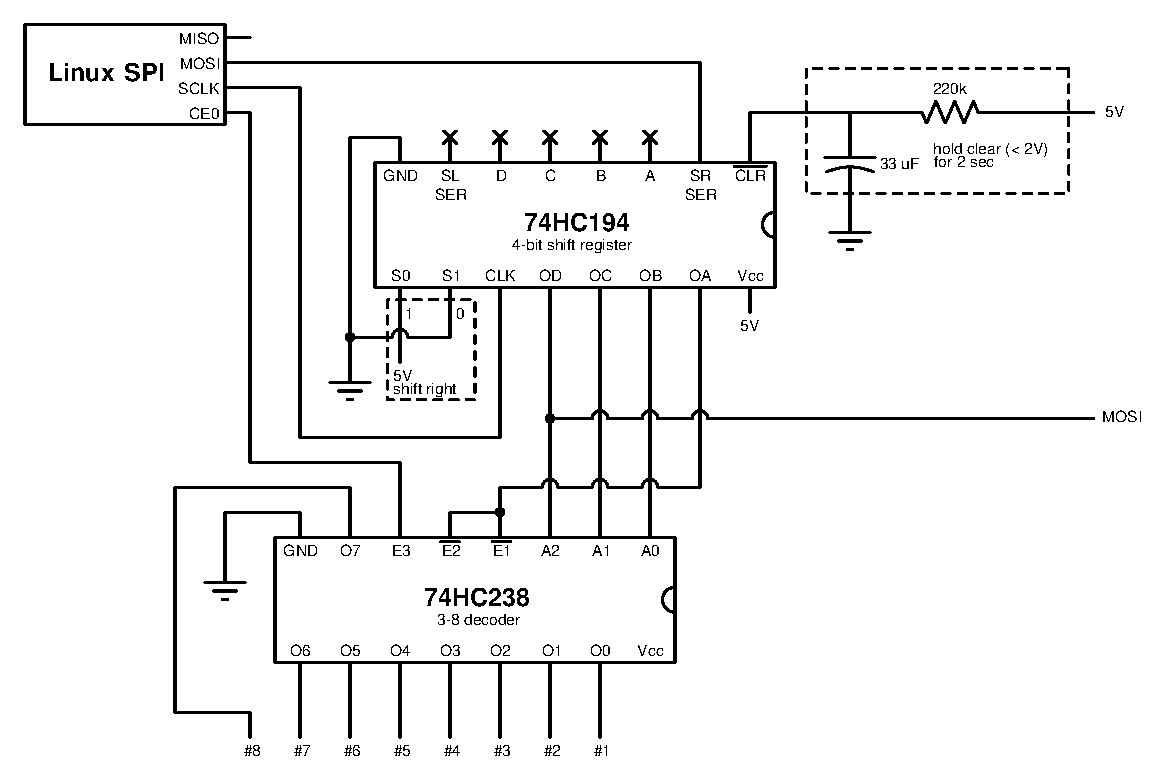
\includegraphics[scale=0.90]{xcircuit/control}
\caption{Sprinkler valve control logic.
Sprinkler valve number is input using SPI from the RasberryPI in
to the shift register.  The number is decoded and inverted to produce
a single high signal for one valve.
All outputs are disabled when OA is clear.}\label{fig:control}
\end{figure}

On power up it is important that the valves remain off.
However the shift register chip (74HC194) does not guarantee
the output state during power up.
To resolve this issue a simple RC circuit is used to to hold the
chip in the clear state for several seconds after power
on (Figure \ref{fig:control}).

% }}}

% {{{ Driver
\clearpage
\section{Driver}
\label{sec:driver}

\begin{figure}[hbp]
\centering
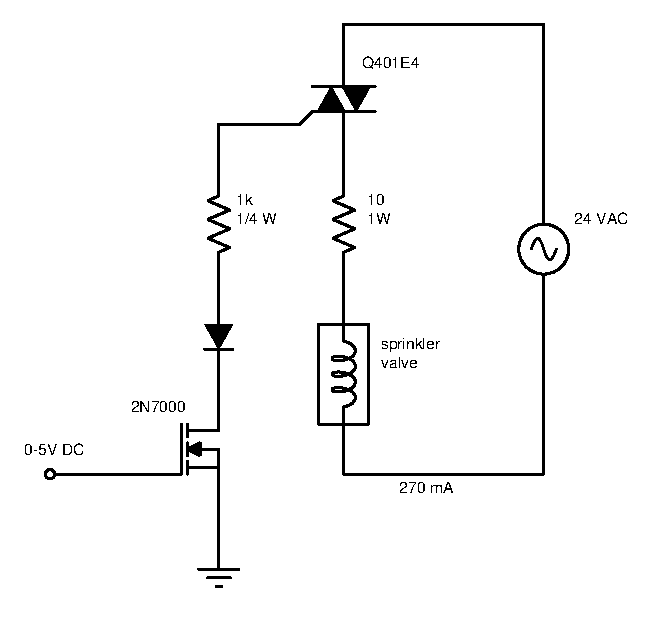
\includegraphics[scale=0.8]{xcircuit/driver}
\caption{Sprinkler valve driver circuit.}\label{fig:driver}
\end{figure}

To turn the sprinkler valves on requires 24 VAC at approximately 270 mA.
If it is assumed that during steady state both the solenoid
and the triac have negligible resistance (Figure \ref{fig:driver}),
a 10 $\Omega$ resistor can be used to limit the current to 240 mA.
At 1 watt the resistor supports the worst case amperage with a margin
over 10\%.

\begin{align*}
	P &= I^2 R \\
	  &= (270\e{-3})^2 \cdot 10 \\
	  &= 0.729 \quad \text{[W]}
\end{align*}

The control signal to the triac (Q401E4) is very sensitive.
The tinyest current will cause it to conduct.
If it is driven by a 0-5V signal it will conduct not only
with a 5V signal but also with 0V signal.
To overcome this issue a diode was used to ensure no current
flows when it is reverse biased.
The FET (2N7000) is used to switch the triac while it also
serves to limit the control current of a 0-5 volt signal
to less than 0.5 mA.
This places the control current well within the limits
of CMOS logic as required by the control chips (Section \ref{sec:control}).

% }}}

% {{{ Power Supply
\clearpage
\section{Power Supply}
\label{sec:power}

The power supply must provide two different voltages.
The sprinkler valves require 24 volts AC and the
RasberrPI requires 5 volts DC.
And it must create these from a 110 volt AC input.

The 24 volts AC can be achieved using a split pole transformer.
The 110 volt AC splits in to two 12 volt AC outputs.
By bridging the center of these two 12 VAC outputs
a combined 24 VAC output is available.

The mean current draw of the RasberryPI 500 mA with a maximum of 1 A
\footnote{The current draw of the RasberryPI was determined experimentally to be 500 mA.}.
This can be supplied by a LM7508 5 volt DC voltage supply
which is capable of a 1 A maximum.
But an AC voltage cannot be supplied to the 7508 directly,
it must be rectified first.

Rectifying of 12 VAC results in approximately 15 VDC.
The 7508 can accept a 20 VDC maximum which is well above 15 VDC.
As an extra measure a capacitor can be placed across the
rectifier output to smooth the voltage peaks.
And a 15k bleed resistor can be added to ensure that the capacitor
will safely bleed down when the system is powered off.

The circuit which achieves all of these design constraints is
shown in Figure \ref{fig:power}.

\begin{figure}[hbp]
\centering
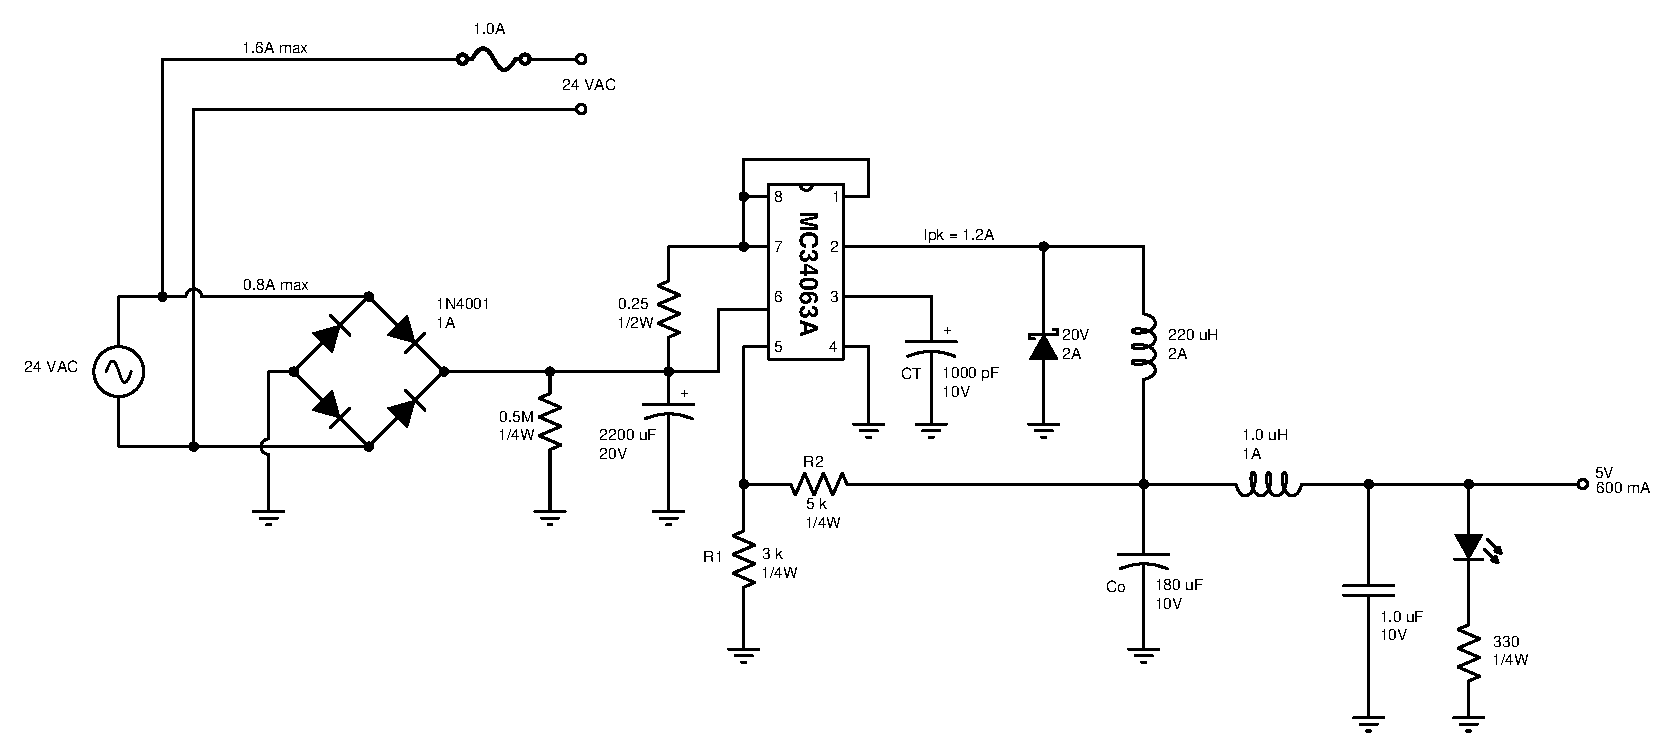
\includegraphics[scale=1.0]{xcircuit/power_supply}
\caption{Power supply circuit.}\label{fig:power}
\end{figure}

% }}}

\pagebreak
\printbibliography

\end{document}
